
\chapter{Podstawy teoretyczne}
\section{Metaverse}


Metaverse to koncepcja w świecie technologicznym, która odnosi się do cyfrowego środowiska życia w którym konwencjonalne struktury społeczne ulegają zmianie. Jest to termin, który łączy w sobie koncepcje greckiego prefiksu „meta”, który oznacza „pełniejszy” lub „przekraczający”, oraz akronimu „Verse” oznaczającego „wszechświat”, który oznacza pojemnik czasoprzestrzenny. Idea metaversum została wprowadzona w powieści science fiction Neala Stephensona \definicja{Snow Crash} w 1992 roku. Szybki rozwój technologii takich jak blockchain, wirtualna (\english{Virtual Reality}) i rozszerzona (\english{Augmented Reality}) rzeczywistość, gry, sztuczna inteligencja i Internet Rzeczy \acronym{IoT} (\english{Internet Of Things}) sprawiły, że metaversum stała się jednym z najbardziej popularnych terminów w świecie technologii. Rozwiązania i usługi są opracowywane dla wirtualnych światów, aby umożliwić użytkownikom dobrą zabawę, inteligentne angażowanie się w otoczenie i nawiązywanie głębszych relacji z innymi użytkownikami \cite{metaverseAsAService}. 

\begin{figure}[htbp!]
    \centering
    \includesvg[width=0.7\textwidth]{images/metaverse/MetaverseInfographic.svg}
    \caption{Koncepcyjny widok metaverse\cite{metaverseUseCaseslee}}
    \label{fig:enter-label}
\end{figure}

Metaverse jako wirtualny świat  wchodzący w interakcję ze światem rzeczywistym i światem ludzkim. Interakcja ta została przedstawiona na rys.\ref{abstractMetaverseArchitectureHumanVirtualPhisical}. Metaverse jest uważany za idealne ucieleśnienie Internetu w przyszłości. Zintegrowany z zaawansowanymi technologiami, metaversum może być wirtualną przestrzenią wzbogaconą o rzeczywistość fizyczną. Użytkownicy są połączeni w wirtualnym wszechświecie we wciągającej interakcji i są ze sobą połączeni w celu prowadzenia działań społecznych. Odkąd koncepcja metaversum została zaproponowana w powieści \definicja{Snow Crash}, ludzie się stopniowo przyzwyczajają do wirtualnych i internetowych aktywności zamiast fizycznych i konwencjonalnych. Odkąd zaproponowano Przemysł 4.0, produkcja przemysłowa przekształca się w kierunku inteligentnej produkcji zwłaszcza w całym cyklu życia produktu, obejmującym badania i rozwój, produkcję, testy i eksperymenty, sprzedaż i transakcje oraz usługi i konserwację. Dzięki zaawansowanym technologiom informacyjno-komunikacyjnym, technologiom rozszerzonej rzeczywistości i sztucznej inteligencji, inteligentna produkcja jest wspierana przez wyższą wydajność produkcji i zwiększoną wirtualną interaktywność użytkowników. Ponadto, jako nowy paradygmat produkcji, produkcja w chmurze wygodnie zapewnia użytkownikom usługi na żądanie. Rozproszone zasoby produkcyjne są wirtualizowane i zarządzane w ujednolicony, zoptymalizowany i konfigurowalny sposób, umożliwiając wysoce wirtualną współpracę i innowacyjną produkcję\cite{industrialMetaverseForSmartManufacturing}. 

\begin{figure}[htbp!]
    \centering
    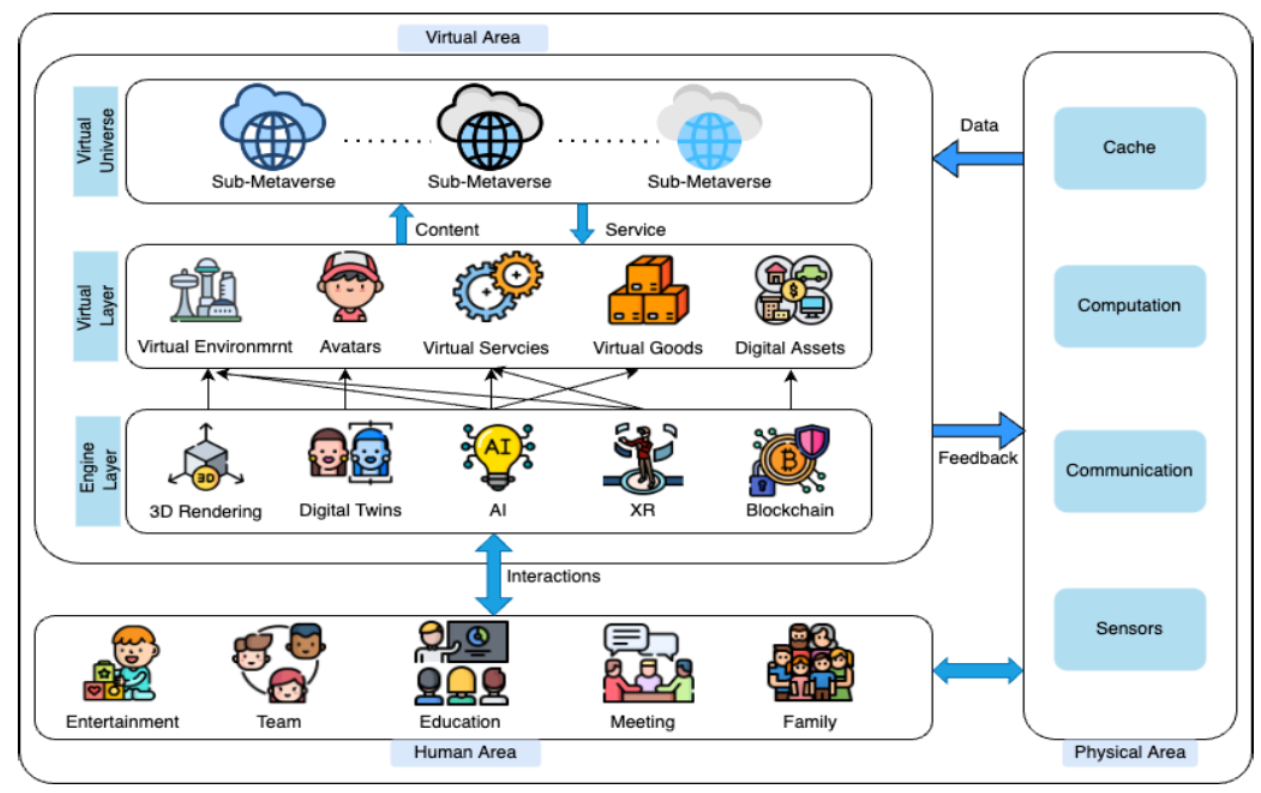
\includegraphics[width=\textwidth]{images/metaverse/metaverseAbstractArchitecture.png}
    \caption{Interakcje w architekturze Metaverse\cite{aSurveyofMobileEdgeComputingForMetaverse}}
    \label{abstractMetaverseArchitectureHumanVirtualPhisical}
\end{figure}

Kluczowe cechy Metaverse:

\begin{itemize}
    \item Trwałość:  oznacza, istnienie niezależnie od fizycznej obecności użytkownika\cite{metaverseAFullDive}.
    \item Nieskończoność: obsługiwanie niezliczonej liczby użytkowników i światów VR\cite{metaverseAFullDive}.
    \item Samowystarczalność: oznacza, że użytkownicy mogą zarabiać w Metaverse i płacić za swoją użyteczność\cite{metaverseAFullDive}.
    \item Interoperacyjność: pomaga użytkownikom przenosić ich wirtualne przedmioty, w tym awatary, z jednego projektu Metaverse do drugiego\cite{metaverseAFullDive}.
    \item Czas rzeczywisty: pozwala użytkownikom cieszyć się doświadczeniami w czasie rzeczywistym\cite{metaverseAFullDive}.
\end{itemize}


Metaverse ma być imersyjnym wirtualnym światem, który płynnie łączy sferę fizyczną i cyfrową, umożliwiając użytkownikom interakcję, współpracę i angażowanie się w szereg działań we wspólnym wirtualnym środowisku. U podstaw tej rewolucyjnej koncepcji leży solidna infrastruktura, która służy jako szkielet, ułatwiając płynną łączność i interoperacyjność. Infrastruktura metaverse to ewoluująca, złożona sieć wzajemnie połączonych technologii, protokołów i ram, które współpracują ze sobą w celu stworzenia jednolitego i spójnego wirtualnego wszechświata\cite{metaverseInfrastructureIEEE}.

Infrastruktura ta obejmuje szeroką gamę komponentów, w tym szybkie sieci, potężne zasoby obliczeniowe, zaawansowane urządzenia sprzętowe i najnowocześniejsze platformy oprogramowania. Wykorzystuje ona najnowsze osiągnięcia w takich dziedzinach jak rzeczywistość wirtualna, rzeczywistość rozszerzona, blockchain i zdecentralizowane przetwarzanie danych, aby zapewnić immersyjne i bezpieczne doświadczenie metaversum użytkownikom na całym świecie\cite{metaverseInfrastructureIEEE}.

\subsubsection{Architektura sieci w metaversum}

Architektura sieci w Metaverse została zaprojektowana tak, aby wspierać płynne interakcje i komunikację w czasie rzeczywistym, umożliwiając użytkownikom angażowanie się w różne działania bez doświadczania opóźnień lub rozłączeń. Wykorzystuje ona zaawansowane protokoły i technologie sieciowe, które priorytetowo traktują niskie opóźnienia, wysoką przepustowość i wydajny transfer danych\cite{metaverseInfrastructureIEEE}.

Zdecentralizowane sieci odgrywają kluczową rolę w zwiększaniu łączności Metaverse. Wykorzystując technologię blockchain i sieci peer-to-peer, infrastruktura Metaverse ma na celu zmniejszenie zapotrzebowania na centralizację zarządców lub pośredników. Takie podejście może zapewnić odporność, przejrzystość i demokratyczne zarządzanie, umożliwiając użytkownikom udział w rozwoju metaversum i procesach decyzyjnych\cite{metaverseInfrastructureIEEE}.

Przesyłanie danych i zarządzanie nimi w ramach infrastruktury Metaverse jest ułatwione dzięki połączeniu tradycyjnych technologii sieciowych i nowych systemów rozproszonych. Szybkie sieci światłowodowe i łączność bezprzewodowa 5G/6G zapewniają przepustowość niezbędną do przesyłania bogatych treści multimedialnych i strumieni danych w czasie rzeczywistym. Jednocześnie zdecentralizowane rozwiązania pamięci masowej, takie jak rozproszone systemy plików i InterPlanetary File System \akronim{IPFS}, zapewniają bezpieczne i redundantne przechowywanie danych, umożliwiając efektywny dostęp do zasobów cyfrowych i ich wyszukiwania\cite{metaverseInfrastructureIEEE}.

Technologie przetwarzania na krawędzi (\english{Edge Computing}) mogą znacząco przyczynić się do zwiększenia wydajności infrastruktury metaverse. Przybliżając zasoby obliczeniowe do urządzeń brzegowych (takich jak zestawy słuchawkowe VR i okulary AR), przetwarzanie brzegowe zmniejsza opóźnienia i poprawia szybkość reakcji, zwiększając ogólne wrażenia użytkownika. Podejście to odciąża również scentralizowane serwery od zadań przetwarzania, rozkładając obciążenie obliczeniowe na całą sieć i zapewniając skalowalność w miarę wzrostu rozmiaru i złożoności metaverse\cite{metaverseInfrastructureIEEE}.

Technologia blockchain może odgrywać kluczową rolę w zwiększaniu bezpieczeństwa sieci w metaversum. Wykorzystując zdecentralizowane mechanizmy konsensusu i protokoły kryptograficzne, blockchain zapewnia integralność i niezmienność danych, chroniąc przed manipulacją i nieautoryzowanym dostępem. Dodatkowo, inteligentne kontrakty ułatwiają bezpieczne i przejrzyste interakcje, automatyzując złożone procesy i umożliwiając transakcje bez zaufania w ramach architektury metaverse i modelowania 3D\cite{metaverseInfrastructureIEEE}.

\subsubsection{Wymagania sprzętowe metaversum}

Aby uzyskać dostęp i w pełni doświadczyć metaversum, użytkownicy będą potrzebować specjalistycznego sprzętu, który może obsługiwać wciągające środowiska wirtualne i płynne interakcje. Podstawą tych wymagań sprzętowych są urządzenia komputerowe, takie jak komputery stacjonarne, konsole do gier lub wyspecjalizowane stacje robocze do rozwoju Metaverse. Urządzenia te muszą posiadać wystarczającą moc obliczeniową, możliwości graficzne i zasoby pamięci, aby renderować szczegółowe środowiska 3D i obsługiwać złożone symulacje technologii Metaverse\cite{metaverseInfrastructureIEEE}.

Infrastruktura Metaverse w dużym stopniu wykorzystuje urządzenia rzeczywistości rozszerzonej i wirtualnej, aby zapewnić użytkownikom wciągające wrażenia. Zestawy VR, takie jak Oculus Rift, HTC Vive i PlayStation VR, przenoszą użytkowników do w pełni zrealizowanych wirtualnych światów, umożliwiając im interakcję z cyfrowymi obiektami i awatarami tak, jakby były prawdziwe. Urządzenia AR, takie jak Microsoft HoloLens i Magic Leap One, płynnie łączą elementy cyfrowe ze światem fizycznym, umożliwiając użytkownikom rozszerzenie otoczenia o wirtualne nakładki i interaktywne interfejsy\cite{metaverseInfrastructureIEEE}.

Zaawansowane jednostki przetwarzające, w tym wysokowydajne procesory graficzne \akronim{GPU} (\english{Graphics Processing Unit}) i wyspecjalizowane akceleratory, odgrywają kluczową rolę w zwiększaniu doznań płynących z Metaverse. Komponenty te są odpowiedzialne za renderowanie złożonych środowisk 3D, symulację fizyki i przetwarzanie ogromnych ilości danych w czasie rzeczywistym. Dodatkowo, integracja sztucznej inteligencji i technologii uczenia maszynowego w infrastrukturze Metaverse wymaga potężnych zasobów obliczeniowych, aby umożliwić inteligentne interakcje, przetwarzanie języka naturalnego i realistyczne awatary\cite{metaverseInfrastructureIEEE}.

Wraz z ciągłym rozwojem technologii, infrastruktura Metaverse dostosowuje się do nowych technologii, które mogą jeszcze bardziej poprawić wrażenia użytkownika. Przykładowo, rozwój interfejsów mózg-komputer \akronim{BCI} (\english{Brain-Computer Interface}) i haptycznych urządzeń sprzężenia zwrotnego może zrewolucjonizować sposób interakcji użytkowników ze środowiskami wirtualnymi, umożliwiając bardziej intuicyjne i wciągające doświadczenia. Co więcej, postępy w dziedzinie obliczeń kwantowych i przetwarzania fotonicznego mogą potencjalnie zrewolucjonizować metaversum, zapewniając bezprecedensową moc obliczeniową a co za tym idzie możliwości przetwarzania danych\cite{metaverseInfrastructureIEEE}.

\subsubsection{Transakcje w metaversum}

Wirtualne waluty i technologia blockchain znajdują się w czołówce, jeśli chodzi o ułatwianie transakcji w Metaverse. Te cyfrowe aktywa, często określane jako kryptowaluty lub tokeny, mogą służyć jako podstawowy środek wymiany towarów, usług i wirtualnych aktywów w wirtualnym środowisku Metaverse. Wykorzystując zdecentralizowany i bezpieczny charakter technologii blockchain, te wirtualne waluty umożliwiają płynne, przejrzyste i pozbawione zaufania transakcje, eliminując potrzebę pośredników i zmniejszając koszty transakcji\cite{metaverseInfrastructureIEEE}.

Inteligentne kontrakty, które są samowykonywalnymi umowami zakodowanymi w sieciach blockchain, mogą odgrywać kluczową rolę w automatyzacji i zabezpieczaniu transakcji w Metaverse. Kontrakty te definiują zasady i warunki różnych umów, takich jak transfery aktywów, umowy o świadczenie usług i rozliczenia finansowe. Po wdrożeniu, inteligentne kontrakty wykonują się automatycznie, gdy spełnione są wcześniej określone warunki, zapewniając przejrzystość, wydajność i niezmienne prowadzenie dokumentacji dla wszystkich transakcji w ramach immersyjnego doświadczenia Metaverse\cite{metaverseInfrastructureIEEE}.

Aktywami cyfrowymi i własnością intelektualną można zarządzać poprzez połączenie technologii blockchain i zdecentralizowanych rozwiązań w zakresie przechowywania. Tokeny niewymienialne \akronim{NFT} (\english{Non-Fungible Token}) mogą być wykorzystywane do reprezentowania unikalnych zasobów cyfrowych, takich jak wirtualne nieruchomości, dzieła sztuki, przedmioty kolekcjonerskie i przedmioty w grze. Tokeny te są przechowywane w sieciach blockchain, zapewniając łatwą weryfikację własności i pochodzenia. Ponadto zdecentralizowane systemy przechowywania plików, takie jak IPFS, umożliwiają bezpieczne i redundantne przechowywanie treści cyfrowych, zapewniając długowieczność i dostępność wirtualnych zasobów\cite{metaverseInfrastructureIEEE}.

Infrastruktura Metaverse może ułatwiać wirtualne rynki i interakcje gospodarcze poprzez integrację zdecentralizowanych aplikacji \akronim{dApps} (\english{Decentralized application}) i zdecentralizowanych protokołów finansowych \akronim{DeFi} (\english{decentralized finance}). Platformy te umożliwiają użytkownikom kupowanie, sprzedawanie, handlowanie i inwestowanie w szeroką gamę wirtualnych aktywów, towarów i usług. Inteligentne kontrakty automatyzują i zarządzają tymi transakcjami, zapewniając uczciwość, przejrzystość i przestrzeganie wcześniej określonych zasad. Co więcej, zdecentralizowane autonomiczne organizacje \akronim{DAO} (\english{Decentralized autonomous organization}) pozwalają na zbiorowe podejmowanie decyzji i zarządzanie w ramach tych wirtualnych rynków, wspierając poczucie wspólnoty i współwłasności\cite{metaverseInfrastructureIEEE}.

\subsubsection{Ekosystem Metaverse}

\begin{figure}[!htbp]
    \centering
    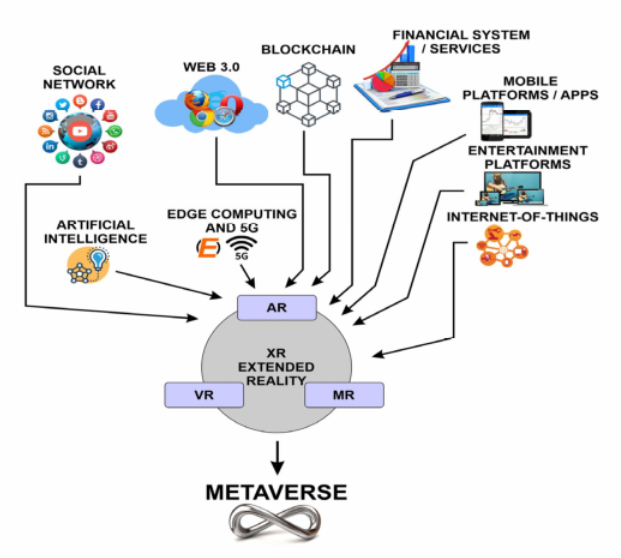
\includegraphics[width=\textwidth]{images/metaverse/metaverseEcosystem.png}
    \caption{Ekosystem Metaverse\cite{metaverseSecurityIssuesChallengesAndViableZTAModel}}
    \label{metaverseEcosystemImage}
\end{figure}

Metaverse umożliwia realizację kilku nowatorskich scenariuszy biznesowych w wielu różnych branżach. Połączenie tych technologii w połączeniu z nowymi rozwiązaniami pomoże zrealizować wizję metaversum w przyszłości. Rys.\ref{metaverseEcosystemImage} przedstawia nadrzędny ekosystem technologiczny umożliwiający powstanie metaversum. Nie ulega wątpliwości, że technologie AR/VR/MR i XR stanowią podstawę metaversum, umożliwiając użytkownikom dostęp do wirtualnego świata 3D . W swojej najwcześniejszej iteracji Metaverse może być zbiorem aplikacji Web 3.0 z XR-Skin zapewniającym ograniczone wrażenia VR. Oczekuje się, że sieci społecznościowe będą jednymi z pierwszych, które przeniosą się do Metaverse, umożliwiając użytkownikom udostępnianie i konsumowanie treści immersyjnych wraz z Web 3.0, umożliwiając firmom oferowanie użytkownikom nowatorskich doświadczeń produktowych. Technologia blockchain zostanie szeroko wdrożona w Metaverse, aby umożliwić realizację wizji zdecentralizowanych finansów i gospodarki twórców, które są nowymi tematami, głównie ze względu na bezpieczeństwo i prywatność, które oferują. Aplikacje i platformy mobilne mogą być kolejnymi, które migrują do Metaverse, a następnie platformy rozrywkowe. Wreszcie, łączność 5G/6G, oferująca niskie opóźnienia, może być spoiwem, które płynnie połączy wszystkie elementy, podczas gdy Internet Rzeczy będzie łączył wszystkie urządzenia wraz z intensywnym wykorzystaniem sztucznej inteligencji, w tym inteligencji brzegowej, w celu zapewnienia spersonalizowanych doświadczeń\cite{metaverseSecurityIssuesChallengesAndViableZTAModel}.


Można przewidzieć, że ekosystem Metaverse przedstawiony na rys.\ref{metaverseEcosystemImage} może przyjąć trzy potencjalne ścieżki ewolucji:

\begin{itemize}
    \item Zamknięty Metaverse: Dla niszowych aplikacji i przypadków użycia ograniczonych do użytku przez konkretną społeczność o wyspecjalizowanych potrzebach.
    \item Federacyjny: Zarządzana i obsługiwana przez dużą korporację z ekosystemem współpracujących partnerów, zewnętrznych dostawców i usługodawców dostarczających użytkownikom końcowym ujednolicone doświadczenie.
    \item Otwarty Metaverse: Metaversum niesfederowana, nie kontrolowana przez żaden pojedynczy podmiot. O otwartej architekturze i społeczności deweloperów tworzących aplikacje/usługi dla użytkowników końcowych.
\end{itemize}



Prawdopodobnym jest, że ekosystem Metaverse, jak pokazano na rysunku \ref{metaverseEcosystemImage}, może przyjąć trzy formy. Można oczekiwać, że wszystkie trzy modele będą współistnieć w takiej czy innej formie. Meta Facebooka jest doskonałym przykładem metaversum federacyjnej\cite{metaverseSecurityIssuesChallengesAndViableZTAModel}. 

Oczekuje się, że w przyszłości pojawią się inne modele, głównie napędzane przez sojusze biznesowe, fuzje i przejęcia. Jest prawdopodobne, że Metaverse napotka kilka przeszkód na drodze do jego szerokiego przyjęcia. Niektóre z wyzwań stojących na drodze do realizacji pełnego potencjału koncepcji Metaverse i jej przyjęcia obejmują:

\begin{itemize}
    \item Dostęp: Obecnie tylko przez zestawy okularów wirtualnej rzeczywistości, które nie są aktualnie powszechne
    \item Łatwość użytkowania: Użytkownicy uważają, że obecna wersja zestawów okularów wirtualnej rzeczywistości jest nieporęczna i trudna do noszenia przez długi czas
    \item Brak rozwiniętego ekosystemu: Niewiele aplikacji dostępnych na obecnych platformach VR
    \item Bezpieczeństwo i prywatność: Środowiska XR cierpią z powodu luk w zabezpieczeniach podstawowych technologii, w tym kwestii dotyczących prywatności użytkowników w wirtualnych światach. 
\end{itemize}

Podczas gdy oczekuje się, że postęp technologiczny rozwiąże kwestie dostępu i łatwości użytkowania w najbliższej przyszłości, kwestie bezpieczeństwa i prywatności muszą być budowane od podstaw podczas projektowania ekosystemu Metaverse\cite{metaverseSecurityIssuesChallengesAndViableZTAModel}. 


\subsubsection{Podsumowanie}

Metaversum stanowi rewolucyjny skok w sposobie, w jaki ludzie postrzegają środowiska cyfrowe i wchodzą z nimi w interakcję, zacierając granice między sferą fizyczną i wirtualną. U podstaw tej koncepcji leży wiele koncepcji solidnej i zaawansowanej infrastruktury, która posłuży jako podstawa płynnej łączności, wciągających doświadczeń i nieograniczonych możliwości. 

W miarę jak metaversum będzie ewoluować i zyskiwać popularność, jej infrastruktura będzie odgrywać kluczową rolę w kształtowaniu przyszłości cyfrowych interakcji, handlu i kontaktów społecznych. Wykorzystując najnowocześniejsze technologie, takie jak blockchain, rzeczywistość wirtualna, rzeczywistość rozszerzona i zdecentralizowane przetwarzanie, infrastruktura Metaverse umożliwia bezpieczne, przejrzyste i interoperacyjne przestrzenie wirtualne.

Pomyślne wdrożenie i rozwój metaversum będzie jednak również wymagać sprostania krytycznym wyzwaniom związanym z zarządzaniem, regulacjami, bezpieczeństwem i prywatnością. Współpraca między zainteresowanymi stronami, w tym deweloperami, decydentami i szerszą społecznością, jest niezbędna do ustanowienia skutecznych ram, które sprzyjają innowacjom, jednocześnie chroniąc użytkowników i utrzymując standardy etyczne.